\vspace{0.25em}

\renewcommand{\thefootnote}{\arabic{footnote}}
\setcounter{footnote}{0}

\chapter*{A Short History of STEDT Software and Database Development}
\addcontentsline{toc}{chapter}{A Short History of STEDT Software and Database Development}

\section{Overview}

The STEDT project spanned a revolutionary period in computer
technology -- from 1987, when (compared to today) very little was possible, and what was
possible normally required a substantial programming team with lots of
experience, to the present, 2015, when everyone is expected to use
computerized devices of several sorts, and  ``collaboration'' and ``data
sharing'' are the norm. Today, databases are everywhere.

The STEDT project at times led the effort and pointed the way in
computational historical linguistics; at other times, it labored to
catch up as the technology ``took off''.

\section{A Timeline}

In 1987, when the STEDT project started, there was no world
wide web. (There was, of course, an internet, but it was restricted to
the military and a few academic institutions.) Only mainframe
computers were connected to each other via networks, and very few
people used email.  Most people used a device called a ``modem'' to ``dial up'' via a
telephone line to access the internet and services. The ability to print specialized characters such as IPA was
limited. Most people were happy that their computer (if they had one)
handled both upper- and lower-case characters.  
Indeed, the ability to make book-quality copy required access to
expensive equipment usually available only to
publishers. PDFs\footnote{Portable Document Format, invented by Adobe
in 1991, but only made opensource in 2008 as ISO 32000 1:2008, and  
so available for use by STEDT. http://en.wikipedia.org/wiki/Portable\_Document\_Format} did not exist, 
nor was it possible to attach a document to an email (one
could, however, ``FTP''\footnote{File Transfer Protocol, RFC114, http://tools.ietf.org/html/rfc114} a file 
from one computer to another, provided the proper software was installed on both sides).

``Microcomputers'', however, did exist, and were becoming ubiquitous -- the IBM PC was becoming standard
office equipment, and the Apple Macintosh\texttrademark had been invented
a few years previously to replace the Apple II and its variations.  
Indeed, the Mac incorporated new-fangled features such
as a {\it mouse}, {\it windows} (movable, resizable ``windows'' on the
screen), and, *gasp* {\it icons}.

And the idea of ``word processing'', the creation and editing of usable
documents using a computer was just becoming a commonly understood
term.\footnote{This term is still in use, but is rapidly becoming
dated. http://en.wikipedia.org/wiki/Word\_processor}

Against this backdrop, the design of a system to create 
the Dictionary-Thesaurus and the gathering and inputting of data supporting
that effort began.  The first bitmap version of
the STEDT font was created, and data was entered into HyperCard\texttrademark stacks.
\footnote{HyperCard was supposed to create a revolution in software
  development, making it possible for ordinary mortals to write their
  own highly interactive applications.}  The project had 3 Mac Pluses\texttrademark, each with a 40MB hard
disk, the maximum possible at that time.  Since there was no
centralized database, software was developed to export the data from the Stacks
into delimited text files which could be combined and sorted into
larger aggregations.

By 1989, a software suite existed, written in Spitbol \footnote{A
  dialect of SNOBOL IV.}, which read the delimited files, sorted the
data (internally), and output ``camera-ready copy'' in
RTF\footnote{Rich Text Format, Microsoft's\texttrademark proprietary markup
  language}.   In addition, a TrueType\texttrademark version of the STEDT font
had been created, enabling the publication of handsome dictionary
pages on the project's newly-acquired PostScript\texttrademark printer, a
LaserWriter\texttrademark.\footnote{Contrast the progression of the
  STEDT project with the development of another similar, but smaller
  effort, the effort to produce the {\it Dictionary of Lahu}. This was
  an early computational lexicographic project of some complexity -- a custom
  font was designed, as well as custom tools for formatting the final
  copy that was reproduced electrographically by UC Press.  The effort
  is handsomely documented in DL and in its derivative the {\it English-Lahu Lexicon}.}

By 1990, the data and analysis supporting what was to be {\it Fascicle
  I: Body Parts} was completed, and it was on this marvelous printer that the
first draft of this fascicle was printed.  By then, a clear picture
had emerged of the requirements of the system: the need to incorporate
several levels of notes and footnotes; the ability to include graphics
(mainly ``semantic flowcharts'') inline; the ``5-level organization''
of the content; the need to (and means to) produce the front-matter
and back-matter associated with the D-T (tables of contents and
figures, indexes of various flavors, and so on.);
and of course the need to be able to iteratively produce, on demand, 
draft versions of the final document for review and revision.  
The essence of this data flow is shown in  Figure~\ref{fig:process1990}.  
The process was a strict file-to-file
pipeline, in which required bits of data were incorporated in several
steps, culminating with a final marked-up document (in this case in
RTF), ready for printing.  

Several ``microcomputer database systems'' became available around this
time. Previous incarnations of these software components (e.g. DBASE\texttrademark) were clunky
and often had restrictions on their ability to handle linguistic data
(as opposed to accounting data).
They handled only short, fixed-length fields, and balked at ``special characters''.

By 1992, STEDT data had been loaded into FoxPro\texttrademark, one of the leading
database systems at that time -- essentially a rewrite of DBASE,
without its many shortcomings, fully relational, with lots of features.
The relational table structure still in use today
was implemented (see Figure~\ref{fig:foxpro}); and the first
``reports'' which allowed users to
browse the growing database were created.  The hardware too was
improving.
Much faster computers with larger hard disks (e.g. the
Apple Quadra\texttrademark) were now connected to each other by Ethernet
cables, and multiple users were able to access the database at the
same time.  A client-server architecture was possible for the first
time.  The ``draft fascicles'' became at this point a type of report
produced by using the database reporting facilities available. While the
reports lacked some of the fine details desired, nay required, for
final publication (e.g. nice footnotes, and inline formatting), the
situation had been infinitely improved by the ability to ``push a
button'' to produce these documents, and the ability for multiple
users to access and update the database at the same time.


\begin{figure}[ht]
\centering
\resizebox{3in}{!}{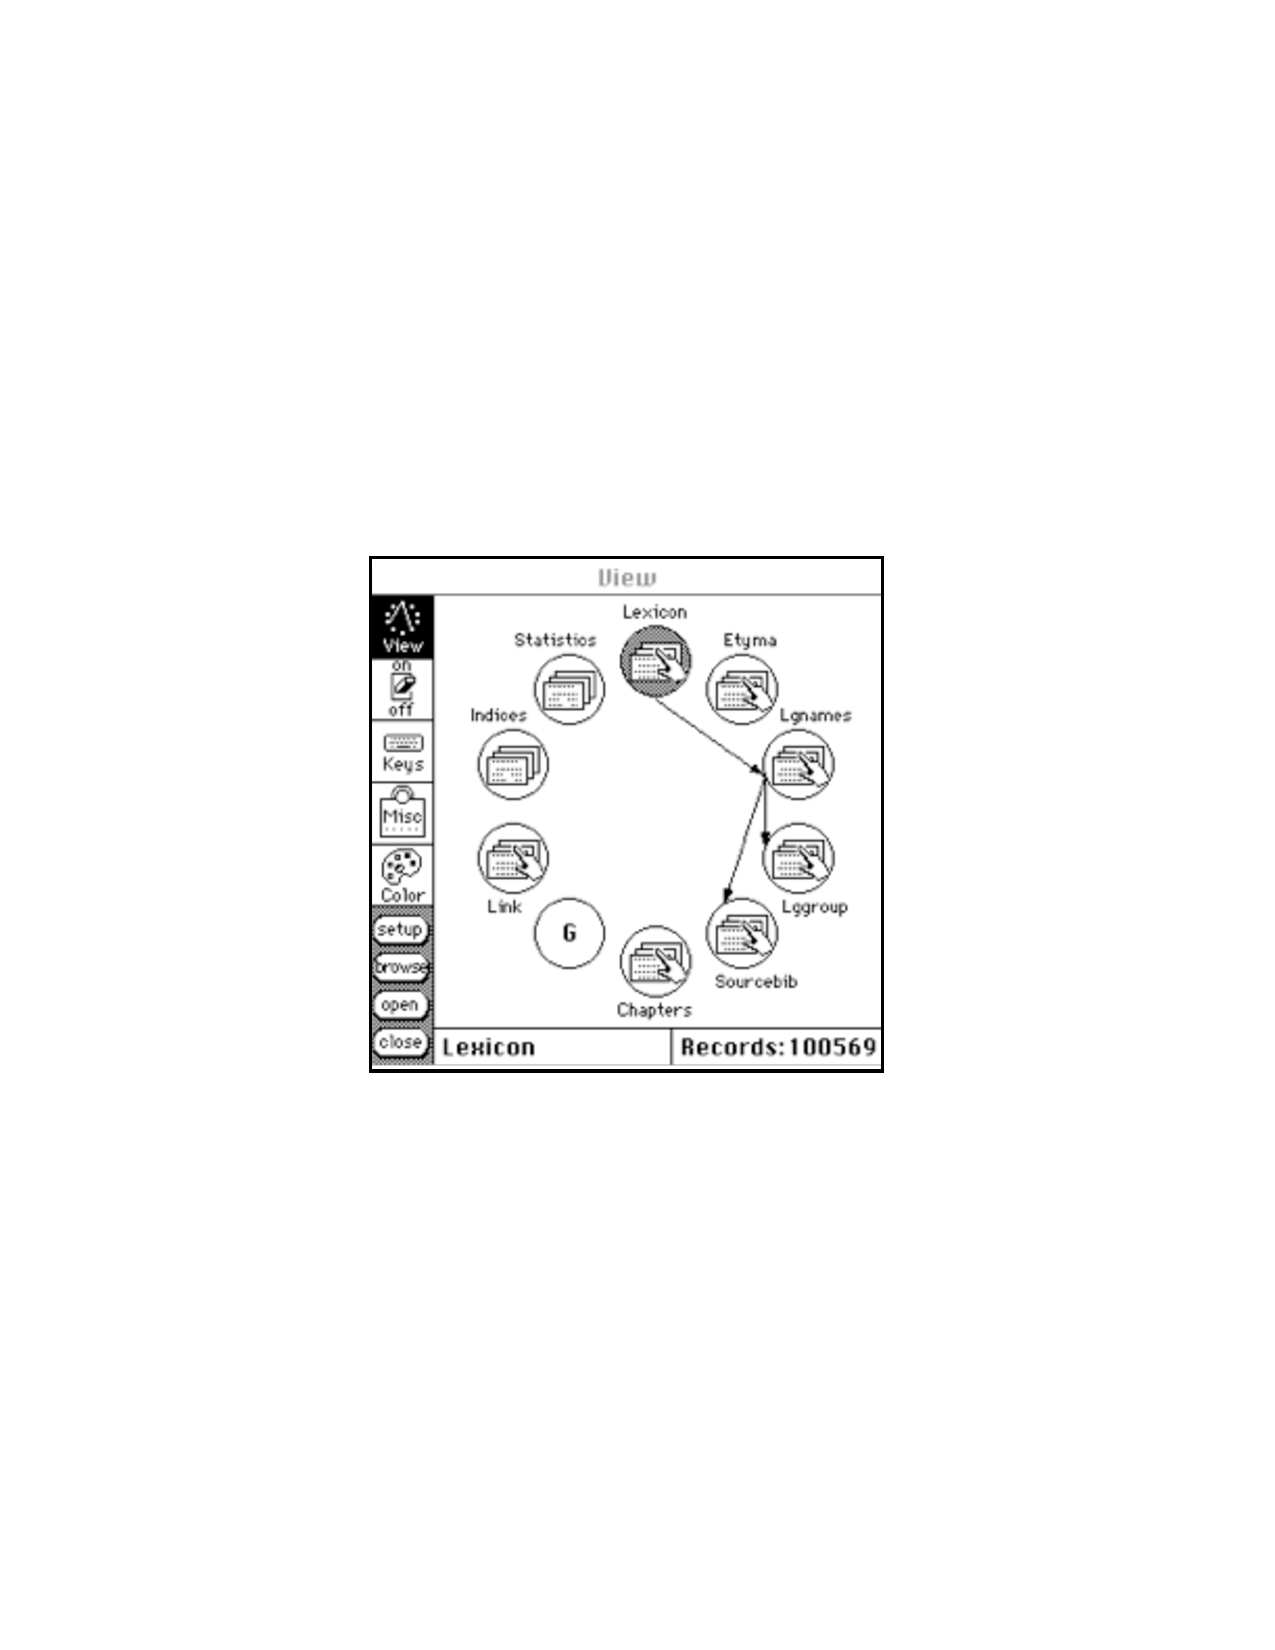
\includegraphics{../../pdf/foxpro.pdf}}
\caption{Relational database layout in FoxPro, circa 1992}
\label{fig:foxpro}
\end{figure}


By 1996, the database had migrated to another database platform,
FileMaker Pro\texttrademark, which had become a popular and flexible system for work
of this sort.   This new technology made it possible to incorporate
data from other database (i.e. FileMaker Pro files) and from other
sources (e.g. images). An elaborate system of linked databases (called
``Ancillary databases'') was produced and operated for some time for
the benefit of the STEDT staff and visitors. However, the system was
never very portable, nor was there a desire to publish these data in
their early and preliminary state. This version remains as a ``legacy
document'' awaiting the attention of a future generation who may wish
to resurrect it from its ashes.

With the advent of the World Wide Web, it became clear that
the STEDT database would eventually need to be available to the world,
and besides, the FileMaker version (absent further programming) was
limited to use in the office; the idea of ``web access'' was very
appealing, as it opened the possibility of having the process of {\it etymologization}
opened up to collaborators all over the world.

Therefore, at the beginning of the 21st century, an effort was made to
migrate the data and software to its current implementation as a
web-based application backed by a powerful database system.  Several
software development iterations (some still operational on the STEDT
website and available in GitHub\footnote{http://github.com/stedtproject} ) were developed.   
The current online application and publication tools are written in PERL,
and run on a so-called ``LAMP stack"��.\footnote{Linux, Apache, MySQL, Perl.}

Today, the STEDT database is freely searchable by anyone anywhere who has
an internet connect web browser.\footnote{http://stedt.berkeley.edu/search.}
In addition, the database itself and
the software used to create the etymological structure and generate
the ``final PDF'' is available as opensource software and open data for the world to
use.\footnote{In a self-referential, or ``meta'' sort of way, it is
  possible to include a link to this {\it final PDF} in this PDF, or
  its printed equivalent, whichever you happen to be reading. The
  link, which will hopefully endure for some time to come is: http://stedt.berkeley.edu/dissemination/stedt.pdf}


\section{Database Design and the Workflow of Etymologization}

\subsection{Supporting the workflow of ``etymologization''}
While the constraints of late 20th-century software and hardware did inhibit some of
the development of the software tools needed to produce the most
compendious of thesauri produced to date, it was the conceptual issues
surrounding the organization of the materials and specifying a robust
and durable workflow that were even more restrictive.  

Beside managing the basic data being input, some means of organizing
it into a semantically-based etymologically-organized whole needed to
be designed and implemented. 

At first, i.e. for the first couple of decades of the project, the
database served the needs of the goal of publishing a
thesaurus. Indeed, to this day, the thesaurus remains the primary
deliverable -- the database and its accoutrements are secondary.

Analyzing the tasks, we noted that producing the dictionary entailed completing at least the following
subtasks:
\begin{itemize}
\item  CREATING A DATABASE:  collecting, evaluating, entering, indexing, and ultimately archiving all significant lexical data available on the Sino-Tibetan languages.
\item  PERFORMING AN ETYMOLOGICAL ANALYSIS OF THE DATA: phonological reconstruction and semantic analysis of the Sino-Tibetan lexicon at various diachronic levels, according to the accepted principles of linguistic reconstruction (i.e. the comparative method).
\item  PREPARING THE DATA FOR PUBLICATION: Several access points must be provided both for the initial data analysis and for the final publication.  Extensive supporting material was required in the form of bibliography, explanations of coding conventions and abbreviations, and other front and back matter.
\item  DISSEMINATING THE RESULTS: the publishing of the physical Etymological Dictionary and
  Thesaurus in two ``tomes".  The promulgation of the database and its
  analysis in machine-readable form for use by other
  scholars in the field.
\end{itemize}


\begin{figure}[ht]
\centering
\resizebox{4in}{!}{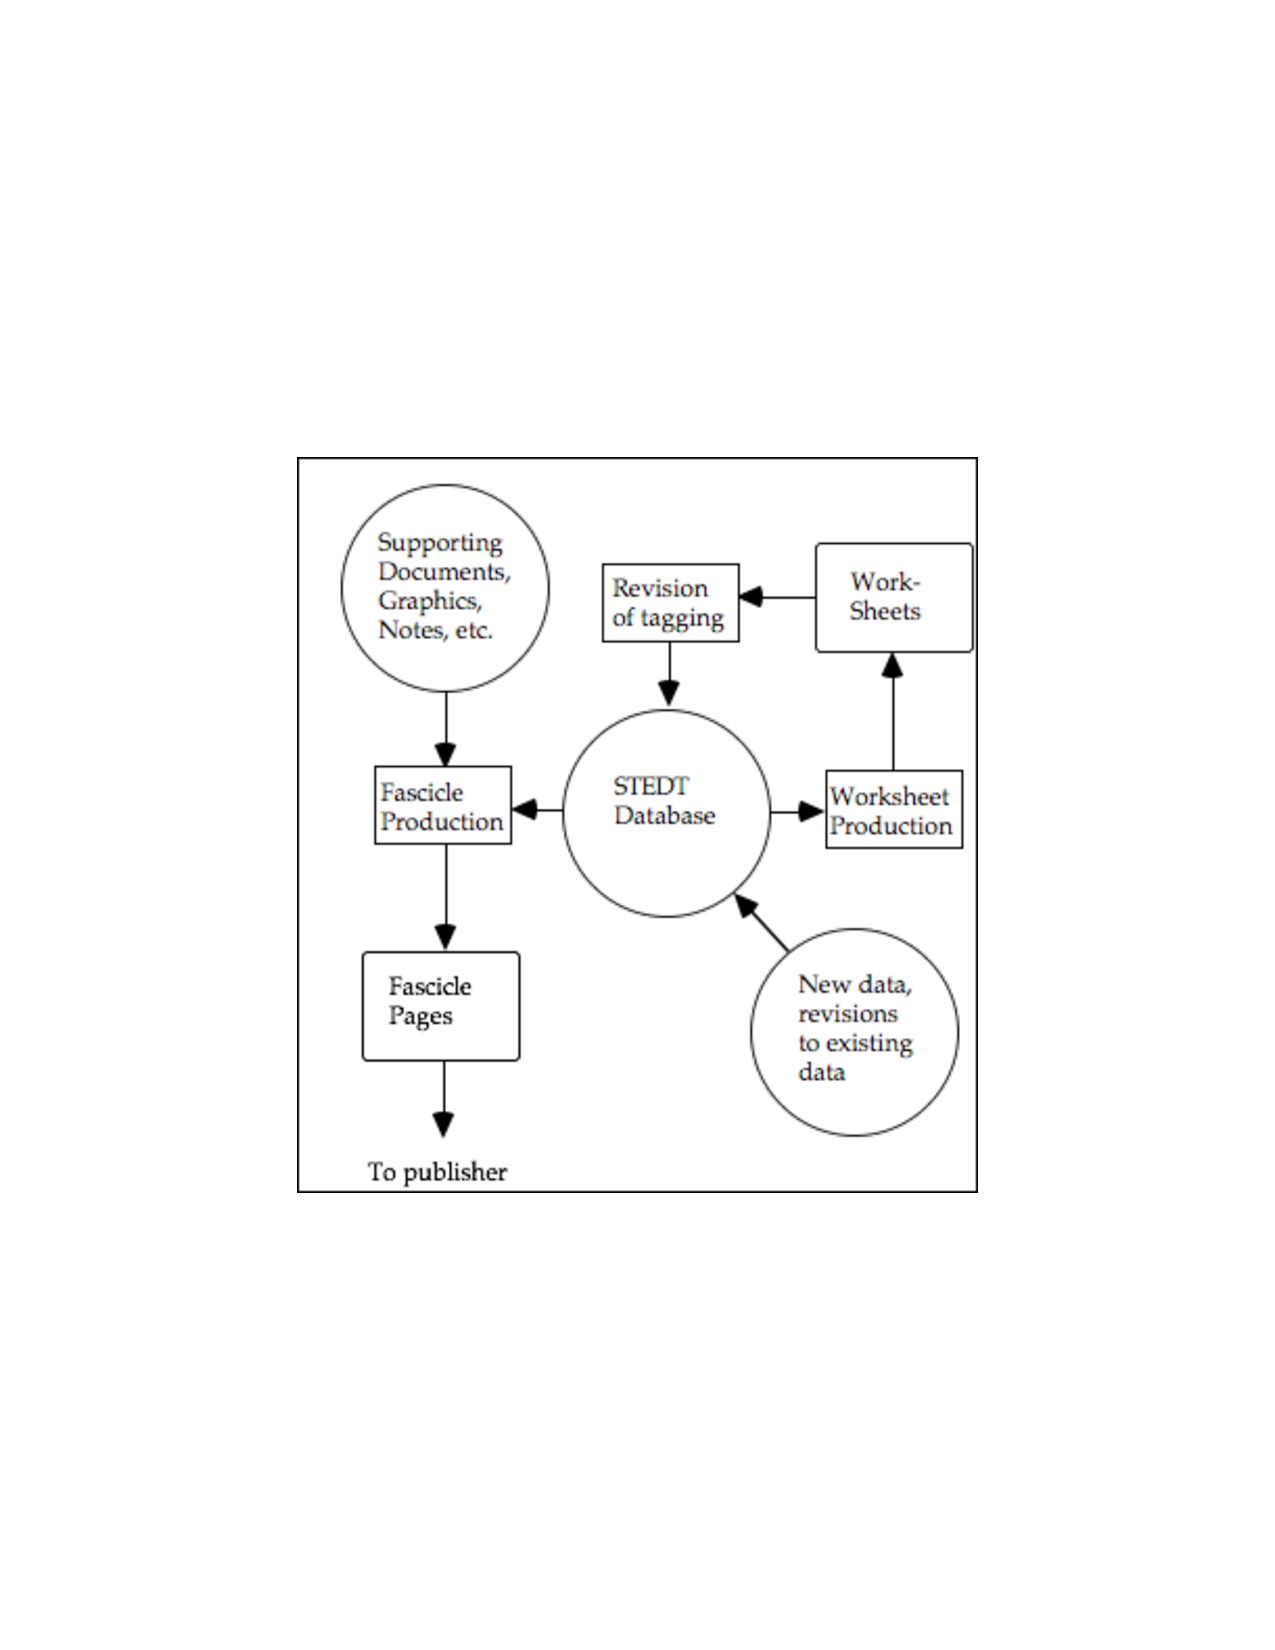
\includegraphics{../../pdf/dataflow1990.pdf}}
\caption{Etymologization and fascicle production, workflow circa 1990}
\label{fig:process1990}
\end{figure}

Each of these tasks required a different approach and skillset. Some
of them (e.g. ``creating a database'') were relatively conventional
and well-understood, if a bit difficult in implement in the
computational milieu at the time.

\subsection{The Invention of ``Tagging"��}
We needed a means, an implementable formalism, to record the
relationship between modern forms and their reconstructed ancestor.
Requirements:
\begin{itemize}
\item  allows marking (extraction) of individual morphemes in modern forms
\item  no specific knowledge of the sound laws required
\item  tolerates phonosemantic variations and accommodates allofamic representations: extrusions, affixes, 
\item  allows flexible (re-)organization of related allofams
\item  quick, easy, intuitive
\end{itemize}


\subsection{Production of the final ``camera-ready" Dictionary-Thesaurus}

The layout of the printed D-T has changed little since it was first conceived of in 1987: Etyma are sequenced within a semantic hierarchy by phonological form and solidity of attestation.  Under each etymon, the supporting forms are listed by language subgroup; within subgroup the forms are ordered by language name and then by gloss.  This is implemented conceptually via a five-level sort key (semantic node, etyma sequence, language subgroup, language name, gloss) associated with each supporting form.   The first version of the D-T was produced by a SPITBOL program which produced MS Word RTF files. These files were edited by hand to include the front and back matter, and to generate a table of contents. The latest and final version of the D-T is generated by a PERL script which extracts sorted data from the database and outputs a series of LaTeX files which are concatenated with front and back matter content to produce a ``master document".  This file is compiled using various LaTeX facilities to produce the table of contents, include the graphic components (mostly semantic flowcharts), the bibliography, and the backmatter indexes.  The process is now fully automatic: a new updated version of the D-T in PDF format is produced nightly. This large document (over 1,000 11"x17" folio-sized pages) can be downloaded and examined at any time.  The nightly file contains the latest database updates and any changes to the front and back matter text that have been checked in to the repository. Thus, the process of producing final camera ready copy is really simply a matter of choosing which nightly version to designate as the final D-T.
A somewhat simplified example of a single cognate set is shown in
Figure 5 below. Note the following significant details of the
arrangement:
\begin{itemize}
\item  The ``5-level sort key" for Milang form shown would be: 
2.1.1+11.00+2.1+Milang+skull
\item  A variety of other material is interpolated into the flow of the text, including notes at various levels, figures and diagrams, and commentary. In this case, a semantic flowchart has been associated with the chapter 2.1.1, and the supporting forms have two footnotes.
\item  The ``cognate morpheme", that is, the portion of the transcribed
  lexical item that is deemed to be distinctly related to the etymon,
  is rendered in boldface -- {\it in the context in which it is cited,
    it is important to note!}
\item  Redundant information, e.g. repeated identical glosses, are elided from the display to increase readability and make the very complex display less busy.
\item  The source of every form cited is included alongside the
form. This is a novel feature of the D-T.
\end{itemize}
As originally conceived, the D-T was to be published as a conventional printed reference work, probably as part of the linguistic series managed the the UC Press.  However, times have changed and the demand for a printed work has diminished; the substantial cost of publishing a work of this sort is now deemed unnecessary: the PDF will be made available publicly, and a few ``reference copies" of the two tome set will be produced for depository libraries, the Library of Congress and a few other interested parties.  The bindery at the UC Berkeley Library has agreed to produce these tomes from the generated PDF at cost, provided a handsome imitation leather cover and a hand-stitched binding.
